\documentclass{exam}

\usepackage{units} 
\usepackage{graphicx}
\usepackage[fleqn]{amsmath}
\usepackage{cancel}
\usepackage{float}
\usepackage{mdwlist}
\usepackage{booktabs}
\usepackage{cancel}
\usepackage{polynom}
\usepackage{caption}
\usepackage{fullpage}
\usepackage{xfrac}
\usepackage{enumerate}
\usepackage{parskip}

\newcommand{\dg}{\ensuremath{^\circ}} 
\everymath{\displaystyle}

\printanswers

% \begin{figure}[H]
%   \centering
%   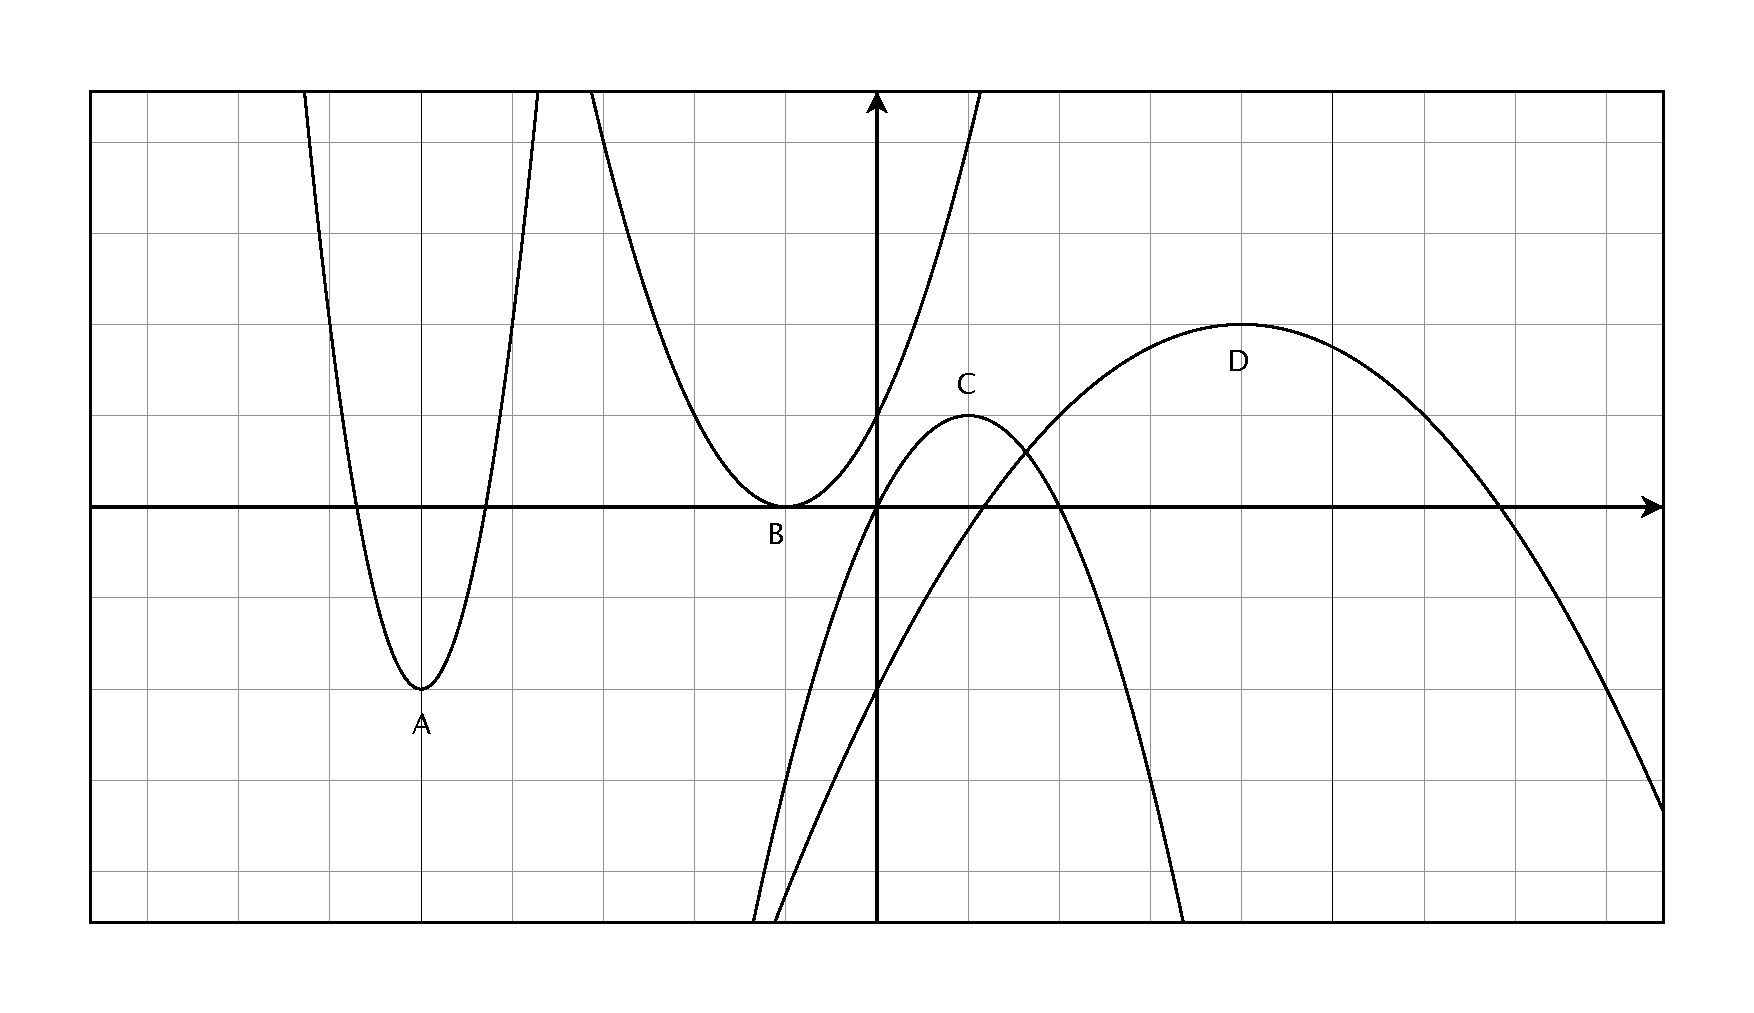
\includegraphics[scale=.3]{problem_7.eps}
%   \caption*{Problem 7}
% \end{figure}

% \begin{tabular}{cc}
% \toprule
% period & amplitude \\
% \midrule
%   $\pi$ & $2$ \\
% \bottomrule
% \end{tabular}

\title{Math 142 Notes \\ Section 6.1}

\date{October 16, 2013}

\begin{document}

  \maketitle
  \tableofcontents

  \section{Exam}
  \begin{itemize*}
    \item review problems from the beginning of the chapter
    \item if you find yourself doing a page of calculations for one problem, you're probably on the wrong track
    \item do in class: 
      \begin{itemize*}
        \item first few problems
        \item word problems
      \end{itemize*}
  \end{itemize*}

  \section{Imaginary Powers of e}

  for large $n$
  \begin{align*}
    e       & \approx \left( 1 + 1/n \right)^n \\
    \\
    e^{1/n} & \approx \left( 1 + 1/n \right)^{n/n} \\
            & \approx 1 + 1/n \\
    \\
    e^{i/1024} & \approx 1 + \frac{1}{1/1024} i \\
               & \approx 1 + 0.0009765625 i \\
    e^{i/512}  & = \left( e^{1/1024} \right)^2 \\
               & \approx 0.999998093 + 0.00195312376 i \\
    \vdots \\
    e^{i} &= 0.540302306 + 0.841470985 i \\
  \end{align*}

  Fill in graphs and plot and find that real part is cosine graph and imaginary part is sine graph:
  \begin{align*}
    e^{i \theta}  & = \cos \theta + i \sin \theta \\
    e^{\pi i}     & = -1 \\
    e^{\pi i} + 1 & = 0 \\
  \end{align*}

  Equation contains all important numbers: $e$, $i$, $\pi$, and $i$.

  \section{Angles}

  Chapter 5 was about repetitive motion (wheels, oscillating springs, pendulums, sound waves).  Chapter 6 is about
  static measurements (distances, construction, surveys, etc.).

  Radians is either:
  \begin{itemize*}
    \item arc length around unit circle
    \item length around any circle divided by the radius.  Circumference is $2 \pi r$--scale by $r$ to get number
      between $0$ and $2 \pi$.
  \end{itemize*}

  Degrees may have came from the approximate number of days in a year or 6 times 60 from Babylonians.

  conversions:
  \begin{itemize*}
    \item degrees to radians: multiply by $\sfrac{2 \pi}{360 \dg}$
    \item radians to degrees: multiply by $\sfrac{360 \dg}{2 \pi}$
  \end{itemize*}

  examples: $30\dg$, $90\dg$, $\sfrac{\pi}{3}$, etc.

  \section{Reference Angle}
  \begin{itemize*}
    \item like reference number from chapter 5
    \item angle between line and shortest route to x-axis
  \end{itemize*}

  \begin{tabular}[H]{lr}
    \toprule
    angle                & reference angle \\
    \midrule
    $45 \dg$             & $45 \dg$ \\
    $150 \dg$            & $30 \dg$ \\
    $370 \dg$            & $10 \dg$ \\
    $\sfrac{3 \pi}{4}$   & $\sfrac{\pi}{4}$ \\
    $\sfrac{23 \pi}{11}$ & $\sfrac{\pi}{11}$ \\
    $31 \pi$             & $\pi$ \\
    \bottomrule
  \end{tabular}

  \section{Coterminal}
  Angles with the same ending line are ``coterminal.''

  \begin{tabular}[H]{lr}
    \toprule
    $45 \dg$             & $-315 \dg$ \\
    $\sfrac{3 \pi}{4}$   & $\sfrac{11 \pi}{4}$ \\
    $- \sfrac{\pi}{4}$   & $\sfrac{7 \pi}{4}$ \\
    \bottomrule
  \end{tabular}

  \section{Arc Length}

  \subsection{Description}
  For a unit circle, the arc length is the same as the angle in radians.  For circle with any other radius, you need to
  scale by the radius to get the arc length.

  \begin{align*}
    \theta & = \frac{s}{r} \\
    s      & = r \theta \\
  \end{align*}

  % \begin{itemize*}
  %   \item find angle in radians
  %   \item multiply by radius
  % \end{itemize*}

  \subsection{Examples}
  \begin{enumerate}
    \item $\theta = \frac{\pi}{5}$, $r = 3$  Find the arc length.
      \begin{solution}
        $s = r \theta = \frac{3 \pi}{5}$
      \end{solution}

    \item $\theta = 135 \dg$, $r = 8$
      \begin{solution}
        convert theta to radians: $\theta = 135 \dg \times \frac{2 \pi}{360} = \frac{3 \pi}{4}$

        find the length: $s = \frac{3 \pi}{4} \times 8 = 6 \pi$
      \end{solution}

    \item How many revolutions of a 24 inch diameter tire to travel one mile?
      \begin{solution}
        The radius is 1 foot.

        \begin{align*}
          C   & = \unit[2 \pi]{ft} \\
          \\
          rev & = \frac{5280}{2 \pi} \\
              & \approx 840 \\
        \end{align*}

      \end{solution}

    \item 
      Seattle's latitude is approximately $48 \dg$ and San Francisco's latitude is approximately $38 \dg$.  How far
      apart are they if Seattle is directly north of San Francisco and the radius of the earth is 3960 miles?
      earth is 

      \begin{solution}
        \begin{align*}
          10 \dg & \approx \unit[0.1745]{rad} \\
          s      & = r \theta \\
                 & = 3960 \times 0.1745 \\
                 & \approx \unit[691]{mi} \\
        \end{align*}

        The actual distance is 800 miles on I-5.

      \end{solution}

  \end{enumerate}

  \section{Sector Area}

  \subsection{Definition}
  Area of circle is $A = \pi r^2$

  Area of quarter circle is $A = \frac{1}{4} \pi r^2$.  Another way of looking at it is:
  \begin{enumerate}
    \item $\theta = \frac{\pi}{2}$
    \item percentage of circle: $\frac{\sfrac{\pi}{2}}{2 \pi} = \frac{1}{4}$
    \item $A = \frac{1}{4} \pi r^2$
  \end{enumerate}

  In general, percentage of circle: $\frac{\theta}{2 \pi}$

  \begin{align*}
    A & = \frac{\theta}{2 \pi} \times \pi r^2 \\
      & = \frac{1}{2} r^2 \theta \\
  \end{align*}

  \subsection{Examples}

  \begin{enumerate}
    \item $r = 2$, $\theta = \frac{3 \pi}{8}$
      \begin{solution}
        \[
          A = \frac{1}{2} 2^2 \times \frac{3 \pi}{8} = \boxed{ \frac{3 \pi}{4} } 
        \]
      \end{solution}

    \item $r = 3$, $\theta = 22 \dg$
      \begin{solution}
        \begin{align*}
          \theta & = 22 \dg \times \frac{2 \pi}{360 \dg} \\
                 & \approx 0.384 \\
          A      & = \frac{1}{2} 3^2 \times 0.384 \\
                 & \approx \boxed{ 1.728 } \\
        \end{align*}
      \end{solution}

    \item $r = 3$, $A = 2 \pi$.  Find $\theta$
      \begin{solution}
        \begin{align*}
          2 \pi  & = \frac{1}{2} 3^2 \theta \\
          % 2 \pi  & = \frac{9}{2} \theta \\
          \theta & = \boxed{ \frac{4 \pi}{9} } \\
        \end{align*}
      \end{solution}
  \end{enumerate}

  \section{Angular Velocity}

  \subsection{Definition}

  \begin{align*}
    v      & = \frac{\Delta s}{\Delta t} \\
    \omega & = \frac{\Delta \theta}{\Delta t} \\
  \end{align*}

  With the same linear velocity, the angular velocity is smaller for large circles and larger for small circles.

  For example, with a circular race track with a 1 mile radius, and a linear velocity of $\unit[100]{mph}$, the
  angular velocity is $\unit[100]{rad/h}$.  
  
  If you increase the radius to 2 miles, it takes twice as long to get around the track since the car now has to
  travel $\unit[4 \pi]{mi}$ instead of $\unit[2 \pi]{mi}$.  The linear velocity is the same, but the angular velocity is 
  now $\unit[50]{rad/h}$.

  In general:
  \begin{align*}
    s      & = r \theta \\
    \omega & = \frac{\Delta \theta}{\Delta t} \\
    \\
    v & = \frac{\Delta s}{\Delta t} \\
      & = \frac{\Delta (r \theta)}{\Delta t} \\
      & = \frac{\Delta r \theta}{\Delta t} \\
      & = r \frac{\Delta \theta}{\Delta t} \\
      & = r \omega \\
    \\
    \omega &= \frac{v}{r} \\
  \end{align*}

  \subsection{Examples}

  \begin{enumerate}

    \item Upgrade tires from diameter $\unit[24.3]{in}$ to $\unit[26.1]{in}$.  How fast is the car now going when the
      speedometer reads $\unit[65]{mph}$ ?

      \begin{solution}
        The speed of the car is the same as the linear speed of a point on the outside of the wheel.  The speedometer
        measures the angular velocity of the wheels.

        \begin{align*}
          \omega & = \frac{65}{r_1} \\
          \\
          v & = r_2 \times \omega \\
            & = \frac{r_2}{r_1} \times 65 \\
            & = \frac{13.05}{12.15} \times 65 \\
            & \approx \unit[69.8]{mph} \\
        \end{align*}

      \end{solution}

    \item NASA has a centrifuge with a 58 foot diameter arm.  They put astronauts on the ends and spin them.  If the
      linear speed of the astronauts is 200 mph, what is the angular velocity of the device?

      \begin{solution}
        \begin{align*}
          r & = \frac{58}{2 \cdot 5280} \\
            & \approx \unit[0.00549242424]{mi} \\
          \\
          \omega & = \frac{v}{r} \\
                 & = \frac{200}{0.00549242424} \\
                 & \approx \unit[36,414]{rad/h} \\
                 & \approx \unit[10.11]{rad/h} \\
        \end{align*}
      \end{solution}

      \item If the device is rotating at 1 rev/s, what is the linear speed of the astronauts?

  \end{enumerate}

\end{document}
